%%%%%%%%%% Basic setup %%%%%%%%%%

\section*{Structure}

Changes are much easier if the construction of the document is structured.
Create a directory named \texttt{img/} to store images and another one named
\texttt{tex/} to store the tex files themselves.

Have a \texttt{main.tex} defining the type of document, title and packages.
This file also calls the tex files from \texttt{tex/}, as well as printing
the bibliography. An example follows:

\inputminted
[
frame=lines,
linenos,
]
{latex}
{main.tex}

The packages are imported in the \texttt{mystyle.sty} file, which reads
(for instance) as follow:

\inputminted
[frame=lines,
linenos,
]
{latex}
{mystyle.sty}

Images like the one shown in Figure \ref{fig:fig} are stored in \texttt{img/}.

\begin{figure}[h!]
    \centering
    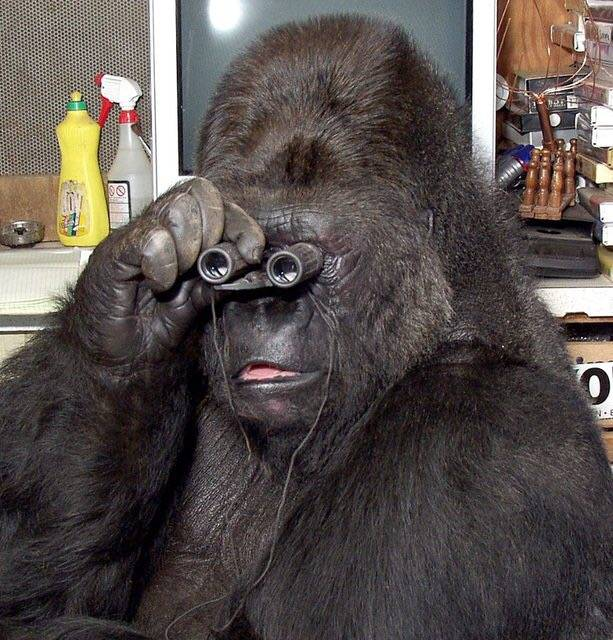
\includegraphics[width=0.5\textwidth]{img/fig.jpg}
    \caption{An image}
    \label{fig:fig}
\end{figure}

The directory \texttt{tex/} on the other hand stores tex files such as this
one (\texttt{basic.tex}), which are loaded using the
\texttt{\textbackslash input\{\}}
command from inside \texttt{main.tex}.  

The bibliography is stored in the bib file \texttt{references.bib}. The
bibliography manager is loaded and references
(such as \cite{nocedal2006numerical}) are added in the last two lines in
the sty file.
